\documentclass[12pt]{article}
%--------------------   start of the 'preamble'
%
\usepackage{graphicx,amssymb,amstext,amsmath,color}
\usepackage[margin=2cm]{geometry}
\usepackage{abstract}
\usepackage{setspace}
\usepackage[footnotesize,bf]{caption}

% TABLE
\usepackage{multicol,hhline,colortbl,multirow}
\usepackage{braket}
\usepackage{siunitx}
\usepackage{hyperref}
\usepackage{authblk}
\usepackage{siunitx}
\usepackage{mathrsfs}
\usepackage[sort&compress]{natbib}
\bibpunct{[}{]}{,}{s}{}{;}


\definecolor{gray}{gray}{0.8}
\def\mobunits{\square\centi\meter\per\volt\per\second}
\def\gcm{\gram\per\cubic\centi\meter}
\def\ccg{\cellcolor{gray}}

\renewcommand{\labelitemii}{$\circ$}
\renewcommand{\bibname}{References}



\title{MorphCT Results - Perfect Perylene Stack}
\author{Matthew Jones}
\date{\today}

\begin{document}
\maketitle

\section{Motivation}

We have observed a difference in charge transport properties for the apparently same morphology, just rotated through some axis such that the columns are either aligned with the box, or antialigned with the box.
This is a problem because nothing about the morphology has changed except the rotation.
We need to:
\begin{enumerate}
    \item{Run a simple system to confirm that rotating the morphology affects the outputs from MorphCT}
    \item{Try to quantify the effect of the rotation on the mobility, anisotropy etc. so that we can account for it (in the perfect world there's some geometric function that we can use based on the anisotropy and direction of the charges to increase/reduce the mobility correctly so that the same morphology always gives the same results)}
\end{enumerate}
If we can solve this, it will be very useful for all of the previous and future work of MorphCT - this has already come up with P3HT and perylene and it will come up with BDT-TPD and honestly anything else that we have that orders into layers.

\clearpage

\section{Mobility Results}


\begin{center}
\begin{tabular}{| c | c | c | c | c | c | c |}
\hline
\rule{0pt}{2.5ex} 
\multirow{2}{*}{\textbf{ID}}&\multirow{2}{*}{\textbf{Morphology Rotation}}&\textbf{Density}&\textbf{Anisotropy}&\textbf{Anisotropy}&\textbf{Stacks}&\textbf{Mobility}\\
                            &&(\SI{}{\gcm})&(Arb. U.)&(Shape)&(Arb. U.)&(\SI{}{\mobunits})\\
\hhline{|=======|}
\textbf{\ccg1}&\rule{0pt}{2.5ex}\ccg 0$^{\circ}$&\ccg 1.14&\ccg 0.9982&\ccg Thin Tube&\ccg9&\ccg7.55$\times 10^{0}$\\
\hhline{-------}
\end{tabular}\label{table:mob}
\captionof{table}{The results from MorphCT for the perfectPerylene crystalline morphology.}
\end{center}

Representative Values From Literature:
\begin{itemize}
    \item{PE Mobility: 2E-1 (one paper reports 5E2)}
\end{itemize}


\clearpage

\subsection{3D Carrier Network}

\begin{figure}[h!]\centering
	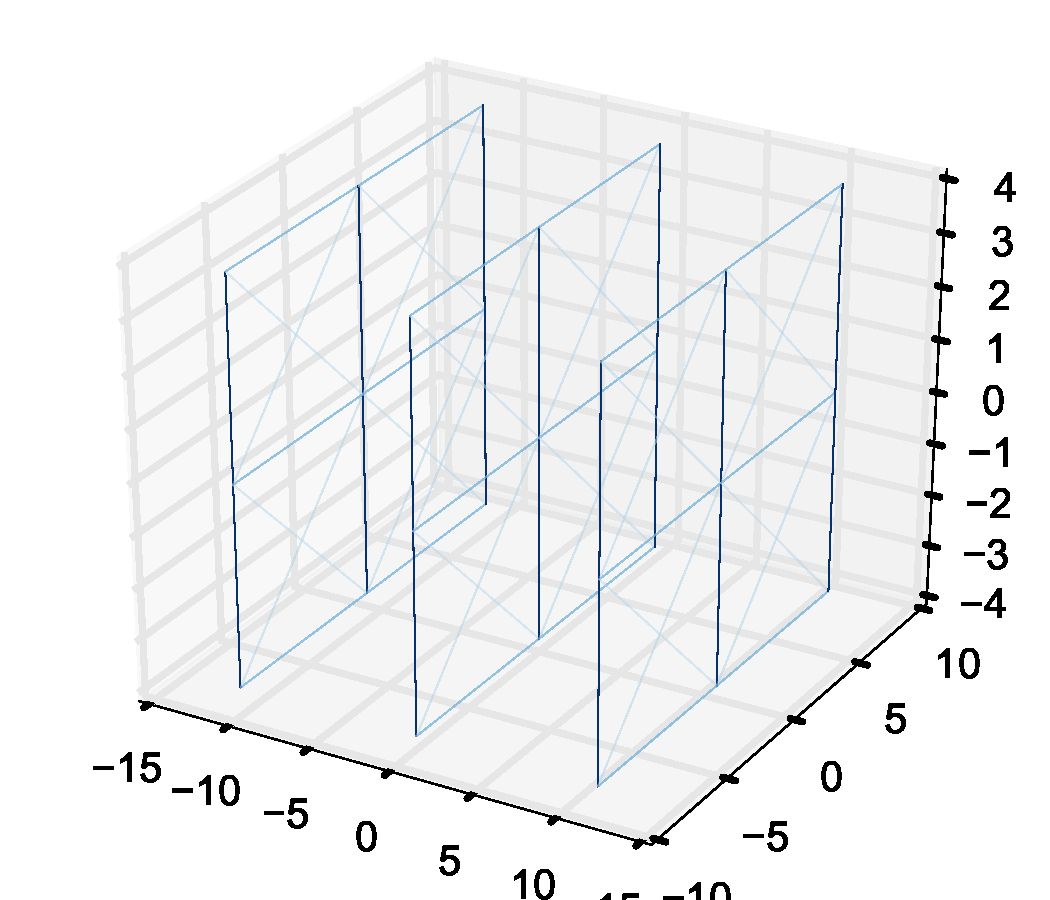
\includegraphics[width=\textwidth]{Figures/3dHole.pdf}
    \caption{The 3D heatmap of charge transport routes within the perfect crystal.
    Dark routes describe commonly accessed hops between pairs of chromophores, whereas pale routes are less widely used in the KMC simulations.
    Each node therefore represents the location of a single chromophore.
The intensity value for the route is currently taken to be \texttt{I $=$ np.log10(freq) $/$ np.log10(max\_freq)}.}
	\label{fig:3dNetwork}
\end{figure}

\clearpage

\subsection{MSDs}

\begin{figure}[h!]\centering
	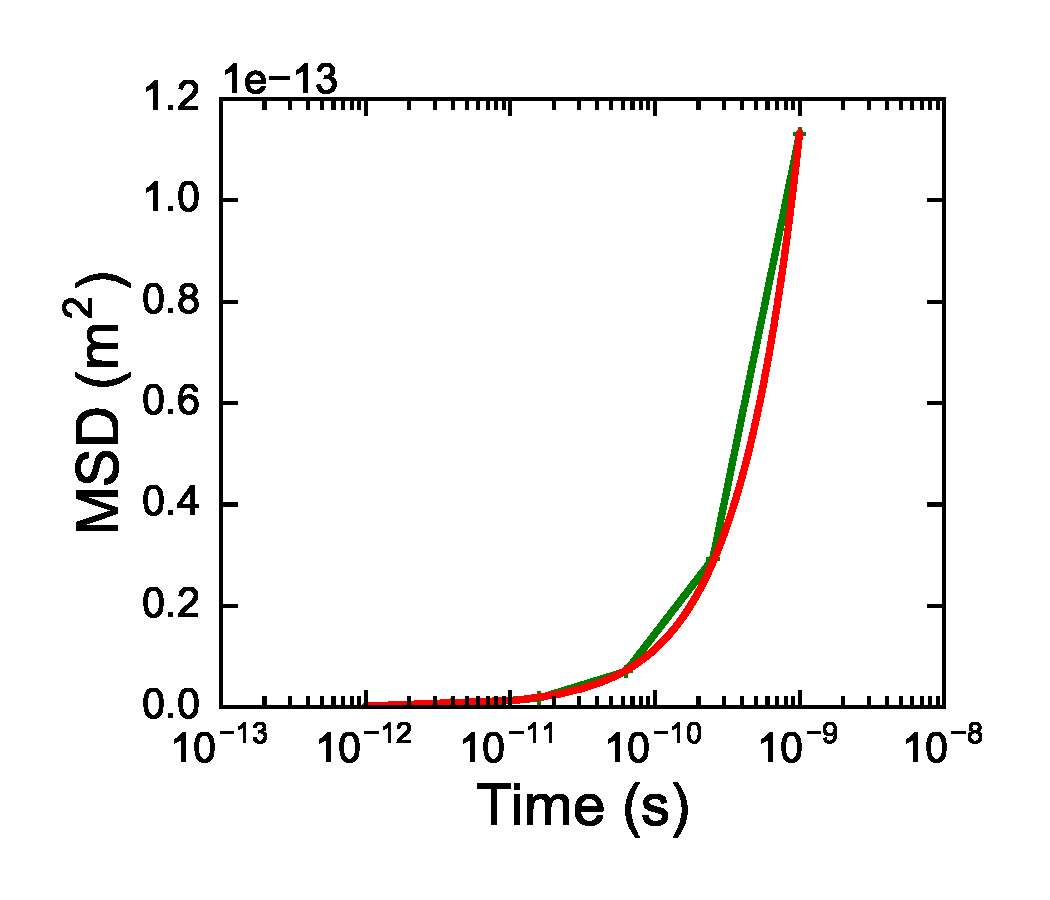
\includegraphics[width=\textwidth]{Figures/SemiLogMSDHole.pdf}
    \caption{The semi-log-x mean squared displacement curves of the carriers within the perfect perylene crystal.}
	\label{fig:MSD}
\end{figure}

\begin{itemize}
    \item{Fitting parameter r = 99.997\%}
\end{itemize}

\clearpage

\subsection{Stacks}

\begin{itemize}
    \item{As before, the chromophores describe individual molecules and not a polymer, and so it makes more sense to consider hops within a stack (intra-stack) and between stacks (inter-stack).}
    \item{Stacks are calculated in the same way as before (see mattySummaries/neatPAHs for more details).}
    \item{As expected, the perfect crystal has 9 stacks.}
\end{itemize}

\begin{figure}[h!]\centering
	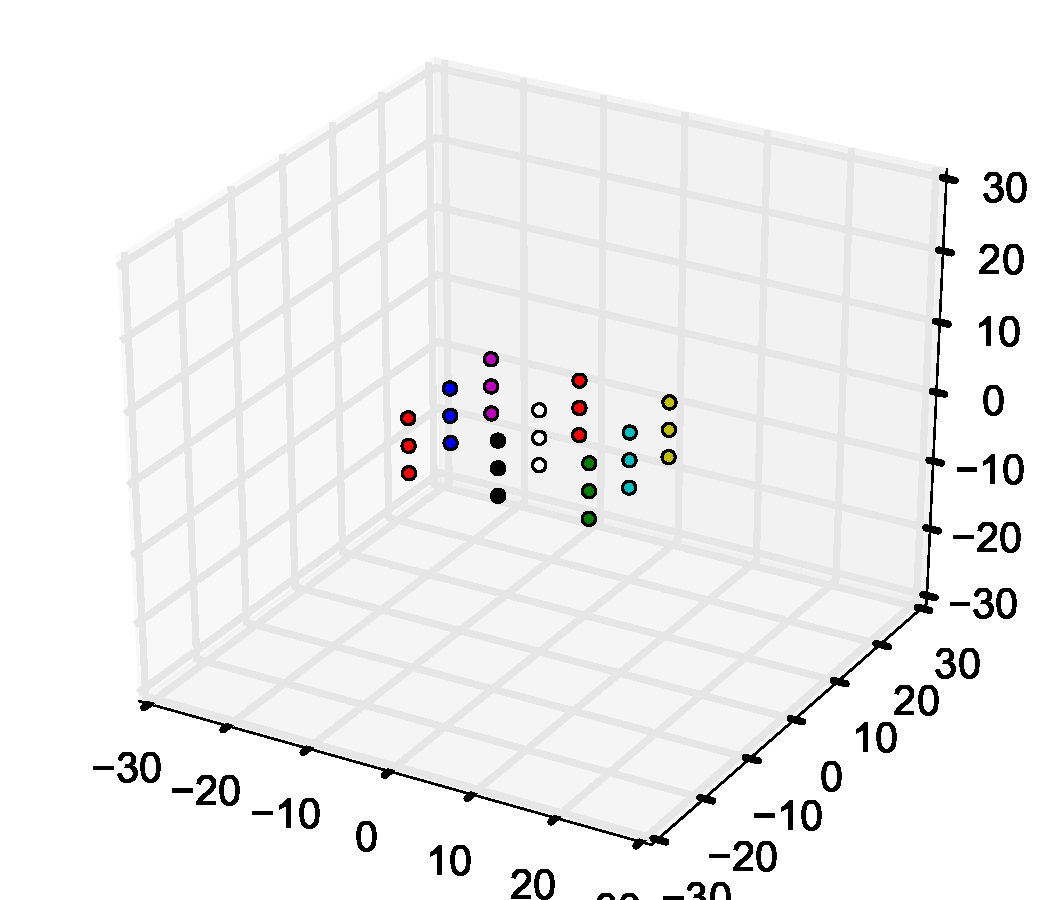
\includegraphics[width=\textwidth]{Figures/stacks.pdf}
    \caption{The 3D visualisations of each stack in the PAH systems. Note: There are 8 basic matplotlib colours, so if $n_{stacks} > 8$, there may be some repeated colours that do not belong to the same stack.}
	\label{fig:stacks}
\end{figure}

\clearpage

\subsection{Hopping Rate Distributions}


\begin{figure}[h!]\centering
	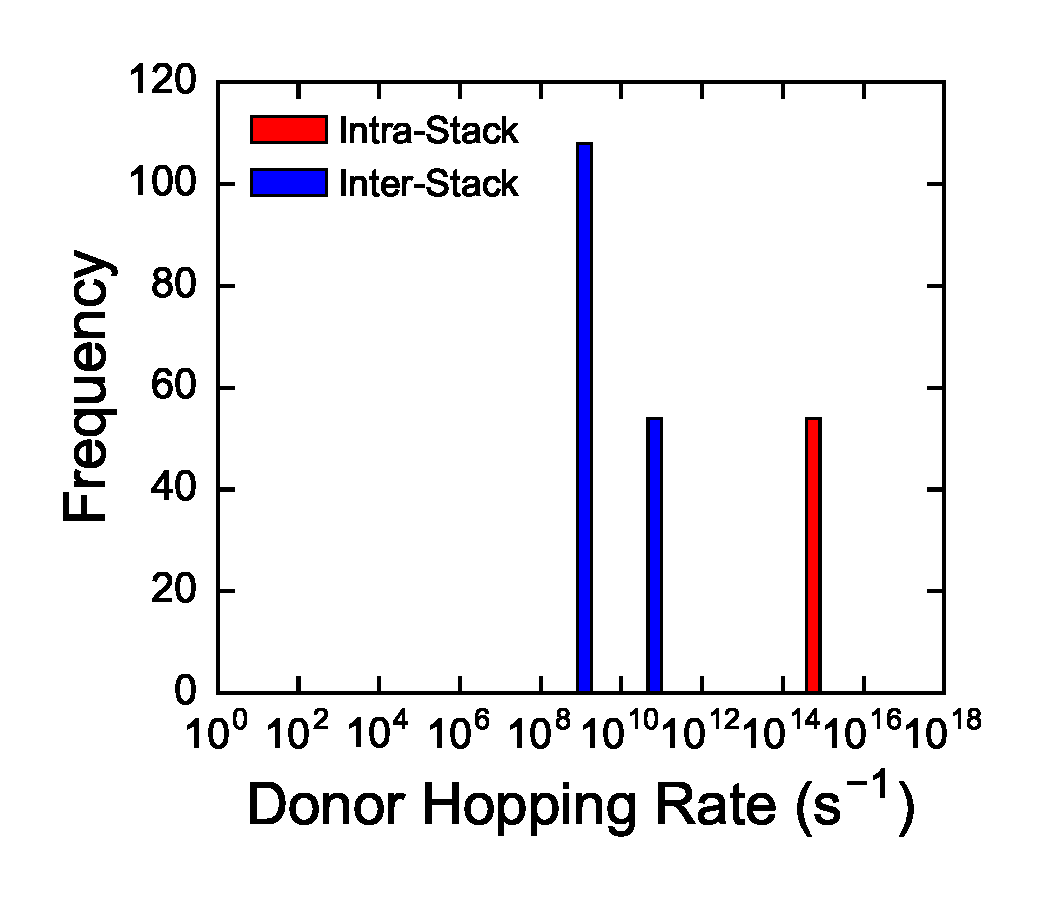
\includegraphics[width=\textwidth]{Figures/DonorHoppingRateMixed.pdf}
    \caption{The hopping-rate distributions for hops executed by carriers within the morphologies \textbf{1} - \textbf{7}. Red bars showhops within the same stack, whereas the blue bars describe hops between stacks. The bars themselves are stacked on top of each other.}
	\label{fig:HoppingRateMixed}
\end{figure}

\bibliography{refs}
\bibliographystyle{unsrt}


\end{document}
